\documentclass[11pt, parskip=half]{scrartcl}
\usepackage{unicode-math}
\setmathfont{TexGyreSchola-Math}
\usepackage{dessertdice}
\usepackage{caption}
\usepackage{ragged2e}

\usepackage[margin=0.43in, paperheight=5.25in, paperwidth=3.75in]{geometry}

% Minimize unwanted hyphenation
\tolerance=1
\emergencystretch=\maxdimen
\hyphenpenalty=1
\hbadness=10000

\usepackage{eso-pic}
\usepackage{booktabs}

\setkomafont{section}{\setmainfont{LondrinaSolid}\LARGE\color{IceCreamPurple}}
\setkomafont{subsection}{\setmainfont{LondrinaSolid}\Large\color{IceCreamPurple}}
\setkomafont{subsubsection}{\setmainfont{LondrinaSolid}\large\color{IceCreamPurple}}

% Adjust spacing before and after section headings
\RedeclareSectionCommand[
  runin=false,
  beforeskip=0.5\baselineskip,
  afterskip=-0.0\baselineskip
]{section}

% Adjust spacing before and after subsection headings
\RedeclareSectionCommand[
  runin=false,
  beforeskip=0.5\baselineskip,
  afterskip=-0.0\baselineskip
]{subsection}

% Adjust spacing before and after subsubsection headings
\RedeclareSectionCommand[
  runin=false,
  beforeskip=0.5\baselineskip,
  afterskip=-0.0\baselineskip
]{subsubsection}


\usepackage{enumitem}

\usepackage[hang,flushmargin]{footmisc}
\newcommand\blfootnote[1]{%
  \begingroup
  \renewcommand\thefootnote{}\footnote{#1}%
  \addtocounter{footnote}{-1}%
  \endgroup
}

\renewcommand{\thefootnote}{\fnsymbol{footnote}}
\renewcommand{\footnoterule}{%
  \kern -3pt
  \hrule width \textwidth height 0.5pt
  \kern 2pt
}

\usepackage[hidelinks]{hyperref}
\usepackage[type={CC}, version={4.0}, modifier={by-sa}]{doclicense} % Add text and icons for creative commons license
%\usepackage{array}

\raggedright
\pagestyle{empty}
\begin{document}

\begin{titlepage}
\AddToShipoutPictureBG{
\begin{tikzpicture}[remember picture, overlay]
%	\node () at (current page.center) {\includegraphics[width=\pagewidth, height=\pageheight]{Images/aloft_cover_background.png}};
	\node () at (current page.center) {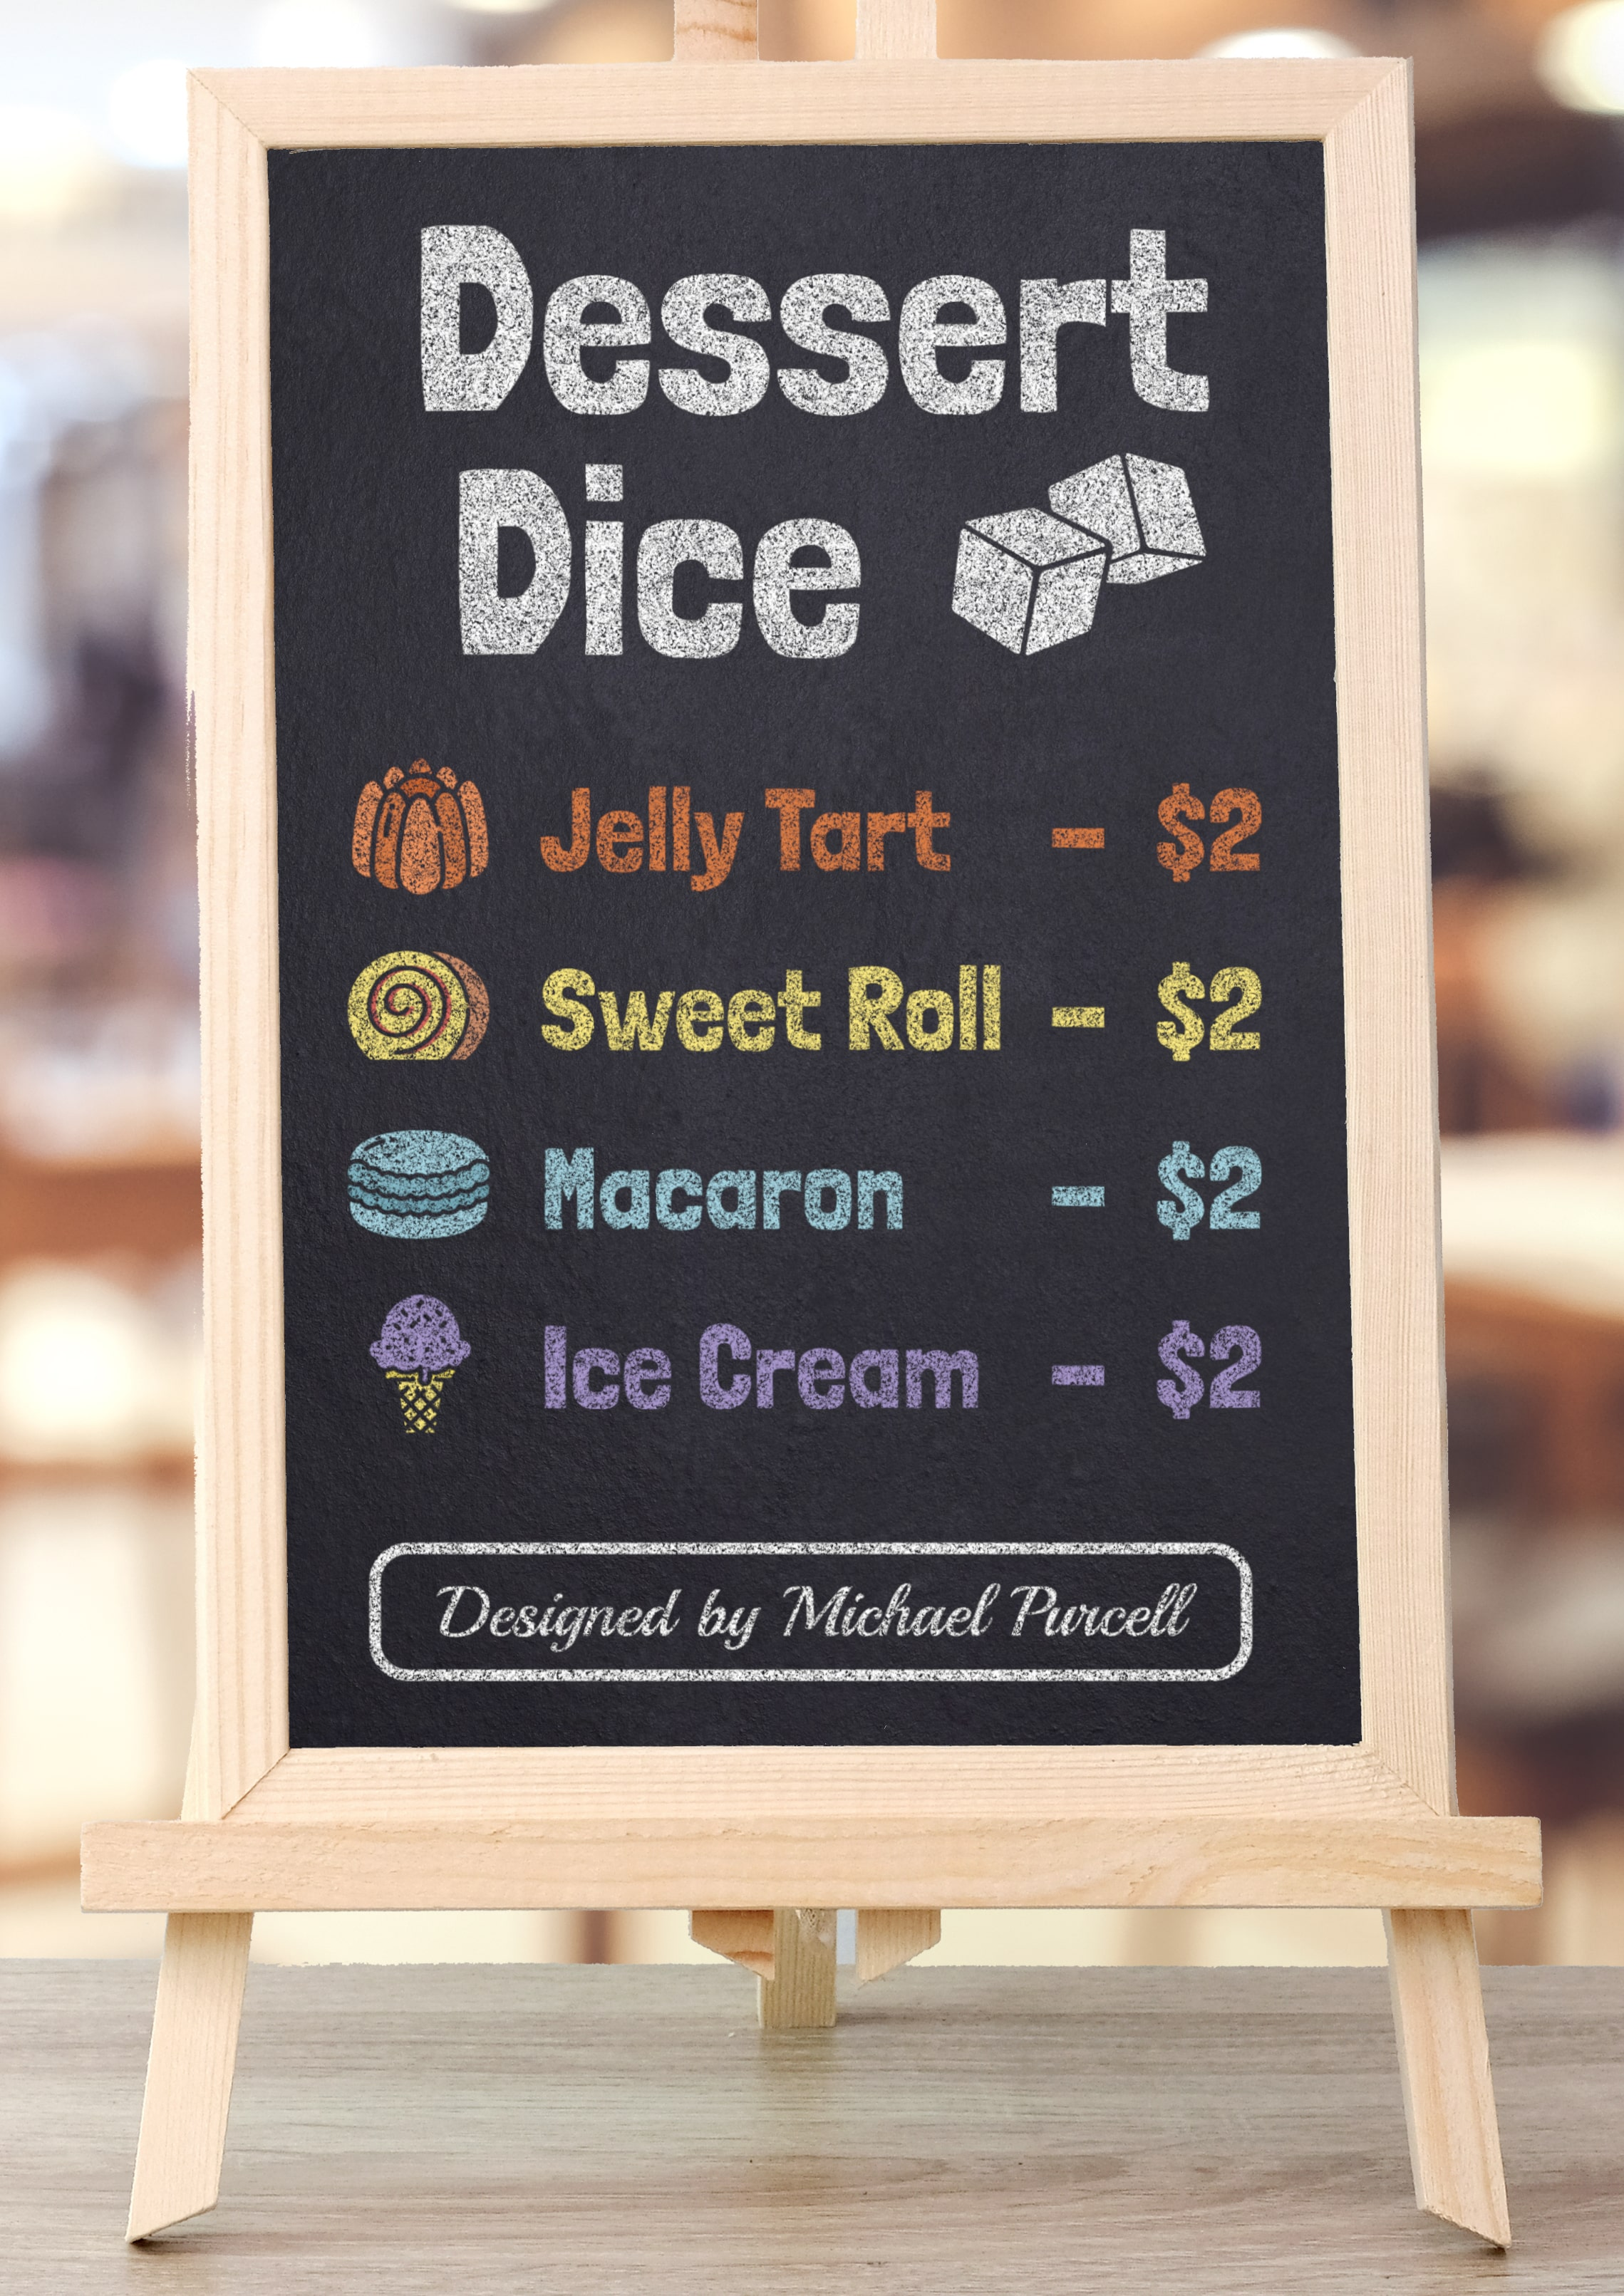
\includegraphics[width=\pagewidth, height=\pageheight]{Images/dessert_dice_front_cover_compressed.jpg}};
\end{tikzpicture}
}

\enlargethispage{3.5\baselineskip}
\setmainfont[Scale=2.75]{LondrinaSolid}
%\setmainfont[Scale=1.9]{LondrinaSolid-Black}
\Huge
\phantom{a}
\end{titlepage}


\ClearShipoutPicture
%\enlargethispage{1.75\baselineskip}
\section*{Components}
\begin{itemize}[leftmargin=*, nosep]
  \item 25 dice
%    \begin{itemize}[nosep, leftmargin=*]
%      \item 6 red dice, 6 yellow dice, 6 green dice, 6~purple dice, and 1 black die.
%    \end{itemize}
  \item 144 stickers
  \item 4 tiles
%      \begin{itemize}[nosep, leftmargin=*]
%      \item 1 Jello Tart card, 1 Sweet Roll card, 1 Popsicle card, and 1 Ice Cream card.
%    \end{itemize}
  \item 1 board
\end{itemize}

\section*{Assembly}
Apply stickers to the dice as follows (the green die should be left blank):

\begin{itemize}[leftmargin=*]
\item \textbf{Orange (6)}: \hfill \raisebox{-1.0ex}{\tikz{\pic {jellyrollicon}} \tikz{\pic {icecreamicon}} \tikz{\pic {macaronicon}} \tikz{\pic {macaronicon}} \tikz{\pic {icecreamicon}} \tikz{\pic {jellyrollicon}}}
\item \textbf{Yellow (6)}: \hfill \raisebox{-1.0ex}{\tikz{\pic {jelloorangeicon}} \tikz{\pic {icecreamicon}} \tikz{\pic {macaronicon}} \tikz{\pic {macaronicon}} \tikz{\pic {icecreamicon}} \tikz{\pic {jelloorangeicon}}}
\item \textbf{Blue (6)}: \hfill \raisebox{-1.0ex}{\tikz{\pic {jelloorangeicon}} \tikz{\pic {icecreamicon}} \tikz{\pic {jellyrollicon}} \tikz{\pic {jellyrollicon}} \tikz{\pic {icecreamicon}} \tikz{\pic {jelloorangeicon}}}
\item \textbf{Purple (6)}: \hfill \raisebox{-1.0ex}{\tikz{\pic {jelloorangeicon}} \tikz{\pic {macaronicon}} \tikz{\pic {jellyrollicon}} \tikz{\pic {jellyrollicon}} \tikz{\pic {macaronicon}} \tikz{\pic {jelloorangeicon}}}
%\item \textbf{Green (1)}: Leave the green die blank.
\end{itemize}

The stickers on opposite faces of every die should match. Three different dessert icons should be be visible regardless of the angle from which any die is viewed.

\newpage
\section*{Overview}
Dessert Dice is a devilishly delicious dice-placement game for two to four players. It can be played in about fifteen minutes and is intended for players who are at least eight years old.

\section*{Set Up}
\begin{enumerate}[leftmargin=*]
  \item Place the board in the play area.
  \item Deal one tile face down to each player. You may look at your tile but you should not show it to anyone else.
  \item Roll all of the dice. These dice comprise the \emph{supply}.
  \item Decide who will take the first turn.\\If in doubt, the person who most recently finished all of their vegetables should go first. 
 \end{enumerate}
 
\newpage
%\enlargethispage{1.75\baselineskip}
\section*{Gameplay}
During the game, you will take turns placing/moving the dice. On your turn you will either place a die from the supply onto the board or move a die from one square on the board to another.

After you take your turn, the player to your left should go next. That is, you should take turns in clockwise order.

The game ends when the board is full. 

\subsection*{Place a Die}
To place a die, take any die from the supply and place it in any empty square on the board.

\begin{itemize}[leftmargin=*]
	\item You may not change which face of the die is pointed upwards (i.e. the die's top face) when you place a die.
\end{itemize}

\newpage
%\enlargethispage{1.75\baselineskip}
\subsection*{Move a Die}
Two squares are \emph{neighbors} if they share an edge. Squares that share only a corner are not neighbors.

To move a die, tip it into an empty neighboring square on the board. Note that moving a die changes both the square the die is in and the face that is pointed upwards.

\begin{itemize}[leftmargin=*]
    \item You may not move a die off of the edge of the board.
    \item You may not move a die diagonally.
    \item If none of a die's neighboring squares are empty, you may not move that die.
    \item You may not undo the previous player's action by moving a die back to the square it was in at the start of their turn.
\end{itemize}

\newpage
%\enlargethispage{1.75\baselineskip}
\section*{Scoring}
The following terminology is used to describe how to compute your score:
\begin{itemize}[leftmargin=*]
	\item A dessert icon is \emph{displayed} on a die if it appears on the top face of that die.% which is pointed upwards.
    \item Two dice are \emph{adjacent} if they are in two neighboring squares on the board.
    \item A \emph{cluster} is a set of dice on which the same dessert icon is displayed and each die in the set is adjacent to another die in the set. 
\end{itemize}

The icon on your tile determines which dice will be used to compute your score.

\newpage
\subsection*{Winning the Game}
Your score is the size of the largest cluster of dice on which your dessert icon is displayed. You win if you have the highest score at the end of the game.

In the case of a tie, everyone should disregard the dice in their largest cluster. Then, recompute your score as the size of the largest remaining cluster on which your dessert icon is displayed.

Continue in this fashion until a winner can be determined. If all of the dice are discarded before determining a winner, then whoever placed the last die wins.



\vfill
\hrulefill

\small
\textbf{Design}: Michael Purcell\\
\textbf{Contact}: \href{mailto:dessert.dice.game@gmail.com}{dessert.dice.game@gmail.com}\\
\textbf{License}: This work is licensed under a\\\phantom{\textbf{License}: }``CC BY-SA 4.0'' license.%\raggedright\doclicenseText
 \newpage
 \AddToShipoutPictureBG{
\begin{tikzpicture}[remember picture, overlay]
%	\node () at (current page.center) {\includegraphics[width=\pagewidth, height=\pageheight]{Images/aloft_cover_background.png}};
	\node () at (current page.center) {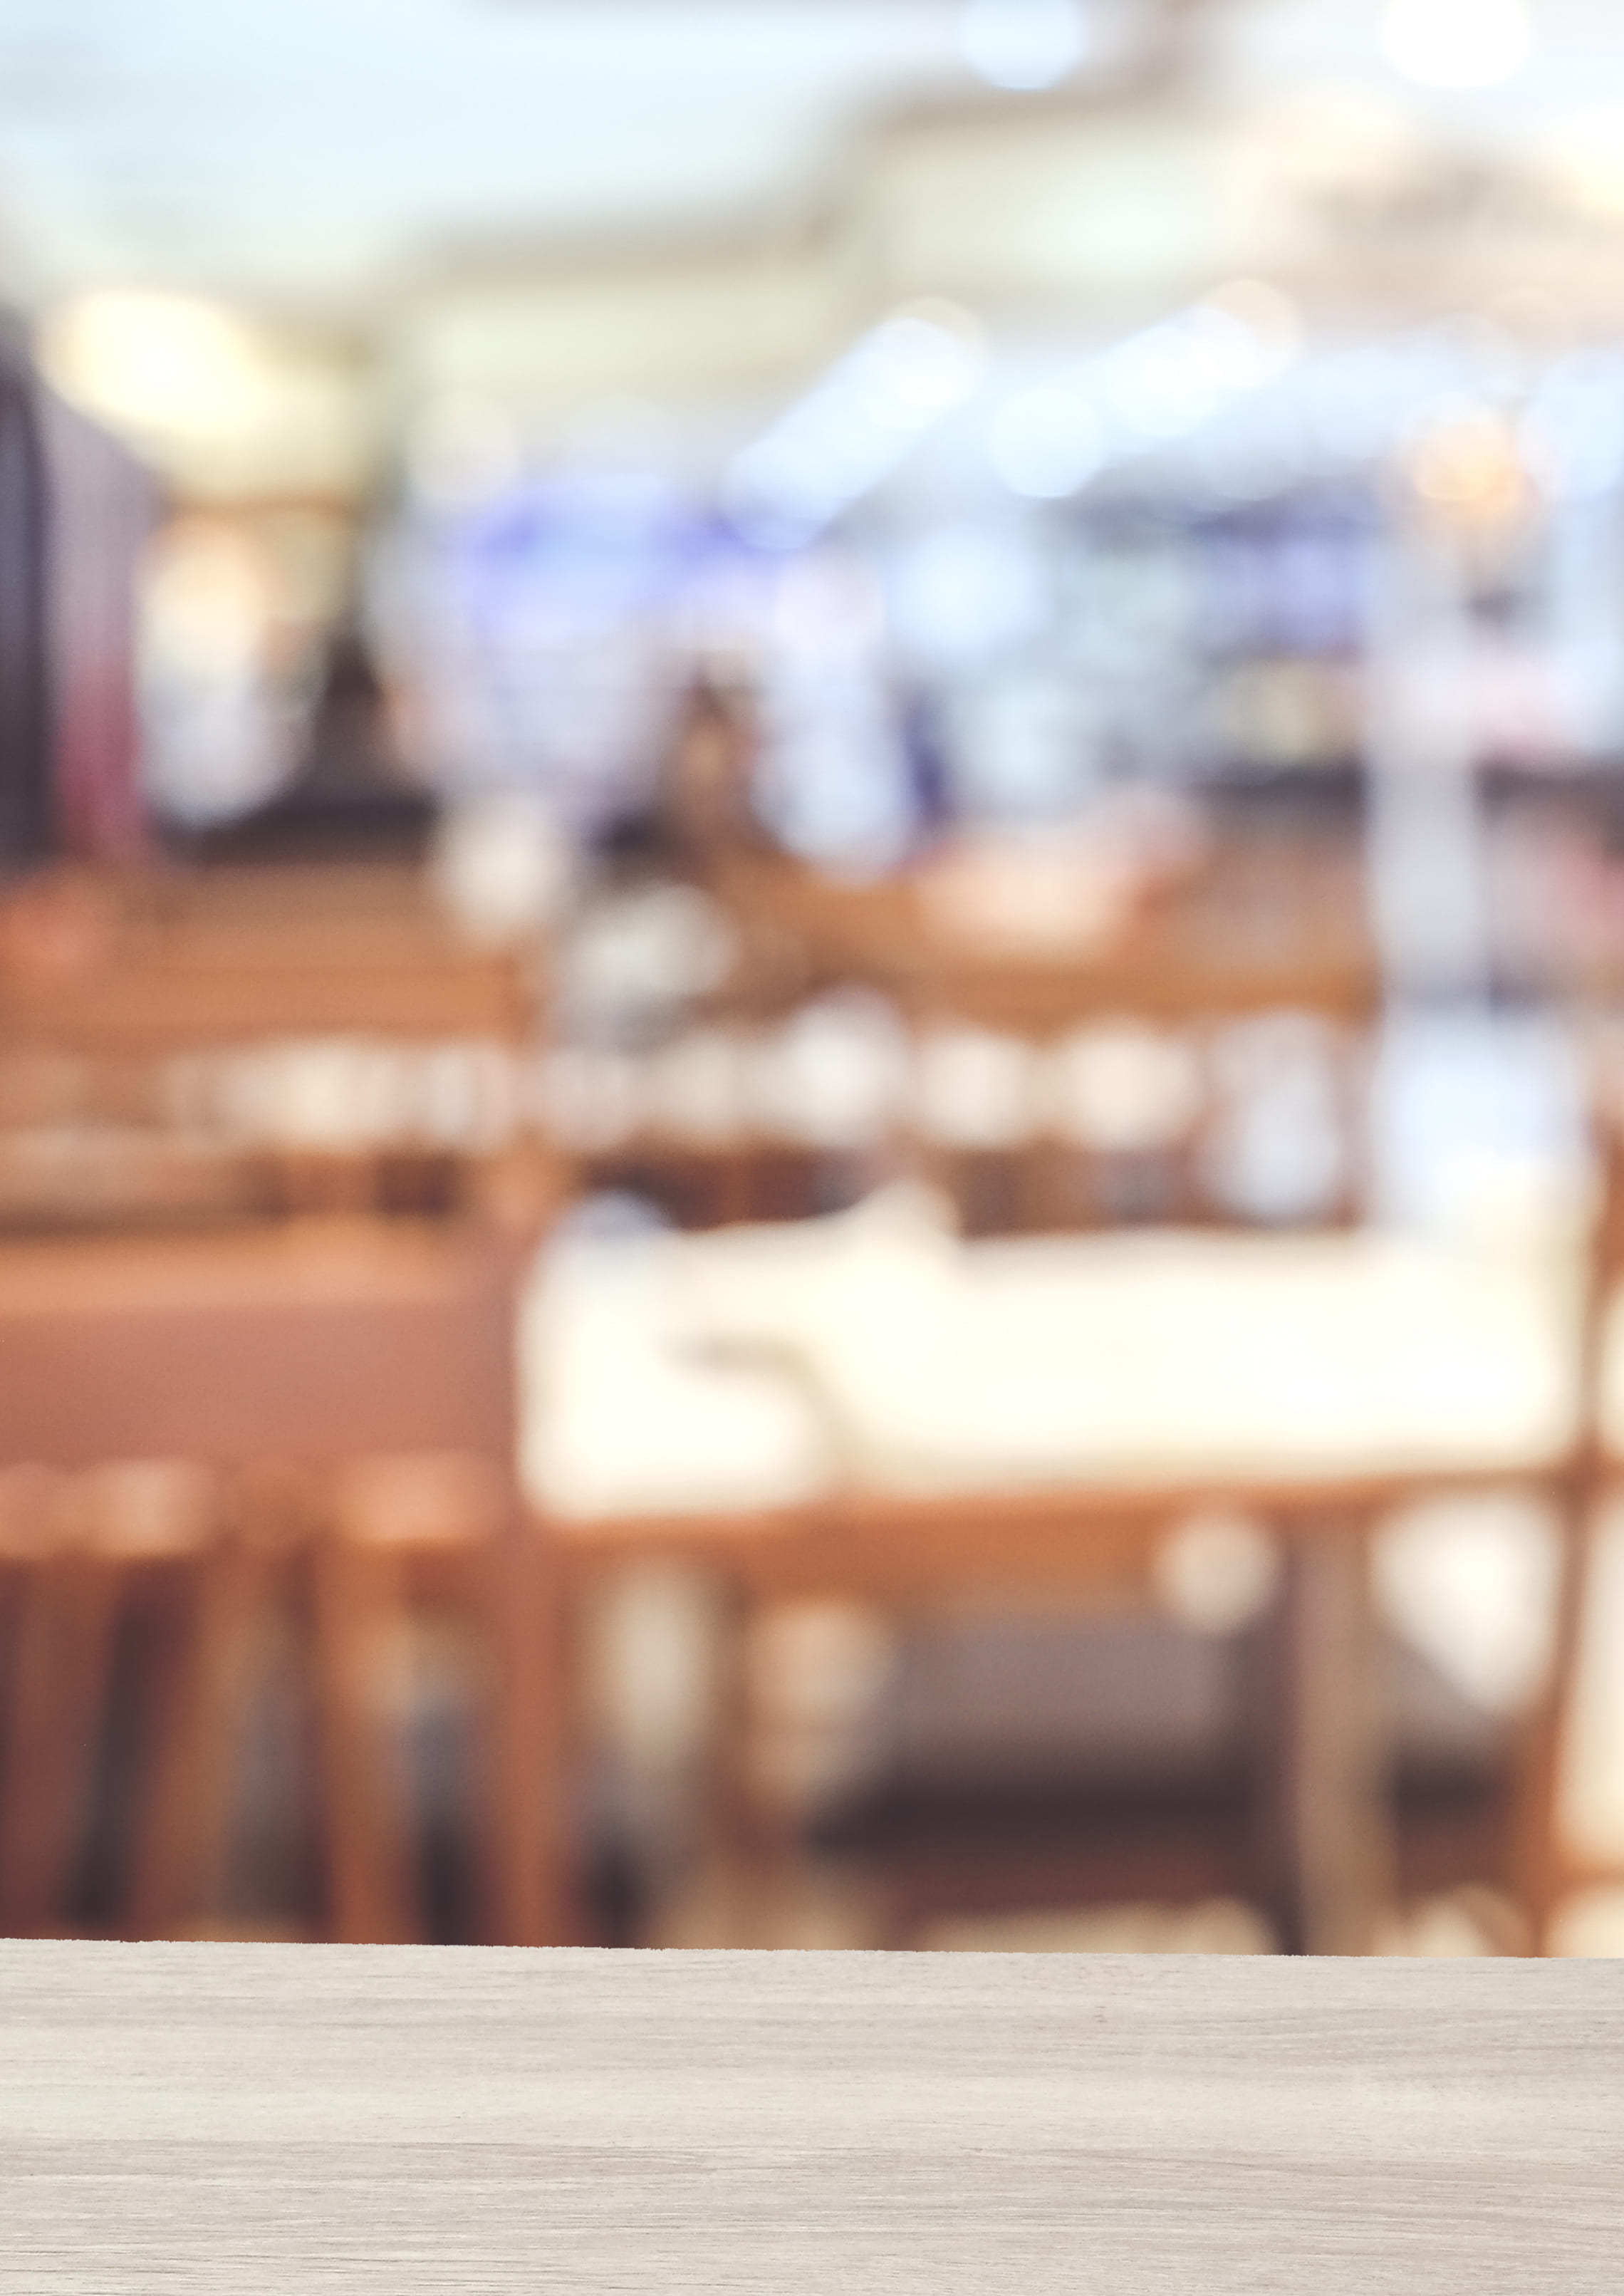
\includegraphics[width=\pagewidth, height=\pageheight]{Images/dessert_dice_back_cover_compressed.jpg}};
\end{tikzpicture}
}
\phantom{Dessert Dice}
\end{document}